\documentclass[12pt]{article}

\usepackage{fullpage}
\usepackage{multicol,multirow}
\usepackage{tabularx}
\usepackage{ulem}
\usepackage[utf8]{inputenc}
\usepackage[russian]{babel}
\usepackage{amsmath}
\usepackage{amssymb}
\usepackage{listing}
\usepackage{graphicx}

\usepackage{titlesec}

\titleformat{\section}
  {\normalfont\Large\bfseries}{\thesection.}{0.3em}{}

\titleformat{\subsection}
  {\normalfont\large\bfseries}{\thesubsection.}{0.3em}{}

\titlespacing{\section}{0pt}{*2}{*2}
\titlespacing{\subsection}{0pt}{*1}{*1}
\titlespacing{\subsubsection}{0pt}{*0}{*0}
\usepackage{listings}
\lstloadlanguages{Lisp}
\lstset{extendedchars=false,
	breaklines=true,
	breakatwhitespace=true,
	keepspaces = true,
	tabsize=2
}
\begin{document}


\section*{Отчет по лабораторной работе №\,3 
по курсу \guillemotleft  Функциональное программирование\guillemotright}
\begin{flushright}
Студент группы М8О-307 МАИ \textit{Безлуцкая Елизавета}, \textnumero 2 по списку \\
\makebox[7cm]{Контакты: {\tt lizabezlutskaya@gmail.com} \hfill} \\
\makebox[7cm]{Работа выполнена: 03.04.2019 \hfill} \\
\ \\
Преподаватель: Иванов Дмитрий Анатольевич, доц. каф. 806 \\
\makebox[7cm]{Отчет сдан: \hfill} \\
\makebox[7cm]{Итоговая оценка: \hfill} \\
\makebox[7cm]{Подпись преподавателя: \hfill} \\

\end{flushright}

\section{Тема работы}
Последовательности, массивы и управляющие конструкции Коммон Лисп.

\section{Цель работы}
Научиться создавать векторы и массивы для представления матриц, освоить общие функции работы с последовательностями, инструкции цикла и нелокального выхода.

\section{Задание (вариант №46)}
Запрограммировать на языке Коммон Лисп функцию, принимающую в качестве единственного аргумента целое число $n$ - порядок матрицы. Функция должна создавать и возвращать двумерный массив представляющий целочисленную квадратную матрицу порядка $n$, элементами которой являются числа $1, 2, ... n^2$, расположенные по спирали.

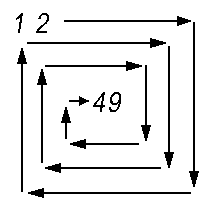
\includegraphics{matrix.png}

\section{Оборудование студента}
Процессор Intel Core i5-3230M 4\,@\,2.6GHz, память: 350Gb, разрядность системы: 64.

\section{Программное обеспечение}
Ubuntu 16.04 LTS, clisp compiler

\section{Идея, метод, алгоритм}
В моём решении матрица условно делится на несколько квадратных рамок, вложенных друг в друга. Делается их обход с самой большой до самой маленькой, где каждая рамка -- это четыре стороны квадрата, которые нужно обойти в направлениях для верхней стороны -- слева-направо, правой стороны --  сверху-вниз и т.д. по кругу.\\

Функция {\tt spiral-matrix} исполняет следующие циклы:
\begin{itemize}
\setlength{\itemsep}{-1mm} % уменьшает расстояние между элементами списка
\item внешний для рамки
\item четыре внутренних для каждой стороны рамки
\end{itemize}

\section{Сценарий выполнения работы}

\section{Распечатка программы и её результаты}

\subsection{Исходный код}

\begin{lstlisting}
(defun print-matrix (matrix &optional (chars 3) stream)
  ;; Предполагаем, что требуется
  ;;  3 знака по умолчанию на каждый элемент,
  ;;  6 знаков на #2A и скобки.
  (let ((*print-right-margin* (+ 6 (* (1+ chars) ; плюс пробел
                                      (array-dimension matrix 1)))))
    (pprint matrix stream)
    (values)))

(defun spiral-matrix (n)
    (let ((matrix (make-array (list n n)))
         (el 1))
    
        (dotimes (i (ceiling n 2))
              (loop for j upfrom i to (- n i 1)
                  do(setf (aref matrix i j) el)
                    (setf el (1+  el))
              )
              (loop for j upfrom (+ i 1) to (- n i 1)
                  do(setf (aref matrix j (- n i 1)) el)
                    (setf el (1+  el))
              )
              (loop for j downfrom (- n i 2) to i
                  do(setf (aref matrix (- n i 1) j) el)
                    (setf el (1+  el))
              )
              (loop for j downfrom (- n i 2) to (+ i 1)
                  do(setf (aref matrix j i) el)
                    (setf el (1+  el))
              )
        )
    
        matrix
    )
)
\end{lstlisting}

\subsection{Результаты работы}
\begin{lstlisting}
(print-matrix (spiral-matrix 1))
#2A((1))
(print-matrix (spiral-matrix 2))
#2A((1 2)
    (4 3))
(print-matrix (spiral-matrix 5))
#2A((1 2 3 4 5)
    (16 17 18 19 6)
    (15 24 25 20 7)
    (14 23 22 21 8)
    (13 12 11 10 9))
(print-matrix (spiral-matrix 7))
#2A((1 2 3 4 5 6 7)
    (24 25 26 27 28 29 8)
    (23 40 41 42 43 30 9)
    (22 39 48 49 44 31 10)
    (21 38 47 46 45 32 11)
    (20 37 36 35 34 33 12)
    (19 18 17 16 15 14 13))
\end{lstlisting}

\section{Дневник отладки}
\begin{tabular}{|c|p{5cm}|p{5cm}|p{3cm}|}
\hline
Дата & Событие & Действие по исправлению & Примечание \\
\hline
03.04.19 & Излишнее использование глобальных переменных & Заменены на локальные переменные & Также внешний цикл был заменен на dotimes и подправлены счётчики во внутренних циклах\\
\hline
&(spiral-matrix 5) возвращает ноль значений & Исправлено (/ a b) на (ceiling a b) & \\
\hline
&(spiral-matrix 5) возвращает ноль значений & Функция spiral-matrix теперь не печатает матрицу, а возвращает её & \\
\hline
\end{tabular}

\section{Замечания автора по существу работы}
Я считаю, что эта задача не очень сложная с алгоритмической точки зрения, но интересная с точки зрения рассмотрения нового языка.

\section{Выводы}
Решая задачи подобного рода, я предпочитаю начинать с рассмотрения частного случая, где выявляется какая-то закономерность. Затем перехожу к выводу формул для общего случая.
\end{document}\grid
\grid
\grid
\grid
